%% rnaastex.cls is the classfile used for Research Notes. It is derived
%% from aastex61.cls with a few tweaks to allow for the unique format required.
\documentclass{rnaastex}

\usepackage{graphicx}
\usepackage[suffix=]{epstopdf}
\usepackage{natbib}
\usepackage{amsmath}
\usepackage{xspace}

% make the word Kepler italicized, deal w/ floating space afterwards
\newcommand{\Kepler}{\textsl{Kepler}\xspace}


\begin{document}


\title{Infrared Flares on M Dwarfs: a Hinderance to\\ Future Transiting Exoplanet Studies}

%% Note that the corresponding author command and emails has to come
%% before everything else. Also place all the emails in the \email
%% command instead of using multiple \email calls.
\correspondingauthor{James. R. A. Davenport}
\email{jrad@uw.edu}

\author{James. R. A. Davenport}
\altaffiliation{NSF Astronomy and Astrophysics Postdoctoral Fellow}
\altaffiliation{DIRAC Fellow}
\affiliation{Department of Astronomy, University of Washington, Seattle, WA 98195, USA}


%% Note that RNAAS manuscripts DO NOT have abstracts.
%% See the online documentation for the full list of available subject
%% keywords and the rules for their use.
\keywords{editorials, notices --- 
miscellaneous --- catalogs --- surveys}



%% Start the main body of the article. If no sections in the 
%% research note leave the \section call blank to make the title.
\section{} 


Dedicated observations by \citet{tofflemire2012} put upper limits on flare flux in the IR for mid-M dwarfs from for moderate amplitude events.

\citet{davenport2012} created peak-flux conversions between $ugrizJHK$-bands for M0--M6, which imply very small amplitudes for IR compared to the dramatic events in the optical.


TRAPPIST-1, a system with 7 transiting exoplanets  (SPITZER DATA) \citep{gillon2017}

K2 data invetigated for transits (LUGER) and flares \citep{vida2017}

%Submissions to RNAAS should be brief communications - 1,000 words or fewer
%\footnote{An easy way to count the number of words in a Research Note is to use
%the \texttt{texcount} utility installed with most \latex\ installations. The
%call  \texttt{texcount -incbib -v3 rnaas.tex}) gives 57 words in the front
%matter and 493 words in the text/references/captions of this template. Another
%option is by copying the words into MS/Word, and using ``Word Count'' under the
%Tool tab.}, and no more than a single figure (e.g. Figure \ref{fig:1}) or table
%(but not both) - and should be written in a style similar to that of a
%traditional journal article, including references, where appropriate, but not
%including an abstract.

Unlike the other journals in the AAS portfolio, RNAAS publications are not
peer reviewed; they are, however, reviewed by an editor for appropriateness
and format before publication. If accepted, RNAAS submissions are typically



%% An example figure call using \includegraphics
\begin{figure*}[h!]
\begin{center}
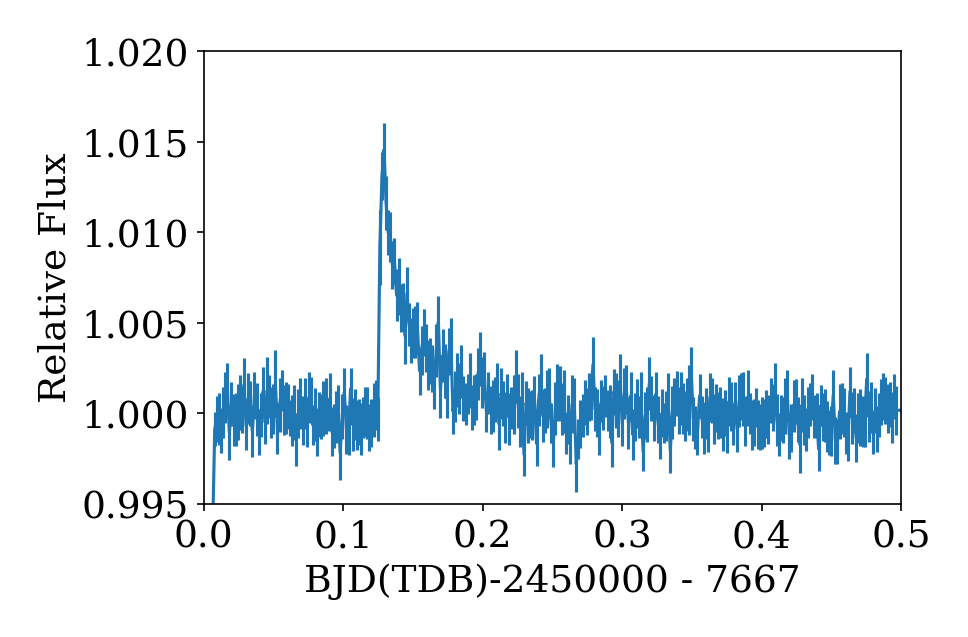
\includegraphics[height=2in]{trappist1_flare3.png}
\includegraphics[height=2in]{flare_17.png}\\
\includegraphics[height=4in]{ffd_ED.png}
\caption{Top: Flares from Spitzer (left) and K2 (right) on TRAPPIST-1. 
Bottom: Cumulative flare frequency distributions for both Spitzer and K2 flare events in units of Equivalent Duration, which can be converted to event energies by 
\label{fig:1}}
\end{center}
\end{figure*}



\acknowledgments

JRAD is supported by an NSF Astronomy and Astrophysics Postdoctoral Fellowship under award AST-1501418. 


%%%%%%%%%%%%%%%%%
\bibliography{/Users/davenpj3/Dropbox/references.bib}

\end{document}
